% Generated by Sphinx.
\def\sphinxdocclass{report}
\documentclass[letterpaper,10pt,spanish]{sphinxmanual}
\usepackage[utf8]{inputenc}
\DeclareUnicodeCharacter{00A0}{\nobreakspace}
\usepackage{cmap}
\usepackage[T1]{fontenc}
\usepackage{babel}
\usepackage{times}
\usepackage[Sonny]{fncychap}
\usepackage{longtable}
\usepackage{sphinx}
\usepackage{multirow}


\title{Introducción al desarrollo de software}
\date{14 de May de 2015}
\release{1.0}
\author{Emiliano López}
\newcommand{\sphinxlogo}{}
\renewcommand{\releasename}{Publicación}
\makeindex

\makeatletter
\def\PYG@reset{\let\PYG@it=\relax \let\PYG@bf=\relax%
    \let\PYG@ul=\relax \let\PYG@tc=\relax%
    \let\PYG@bc=\relax \let\PYG@ff=\relax}
\def\PYG@tok#1{\csname PYG@tok@#1\endcsname}
\def\PYG@toks#1+{\ifx\relax#1\empty\else%
    \PYG@tok{#1}\expandafter\PYG@toks\fi}
\def\PYG@do#1{\PYG@bc{\PYG@tc{\PYG@ul{%
    \PYG@it{\PYG@bf{\PYG@ff{#1}}}}}}}
\def\PYG#1#2{\PYG@reset\PYG@toks#1+\relax+\PYG@do{#2}}

\expandafter\def\csname PYG@tok@gd\endcsname{\def\PYG@tc##1{\textcolor[rgb]{0.63,0.00,0.00}{##1}}}
\expandafter\def\csname PYG@tok@gu\endcsname{\let\PYG@bf=\textbf\def\PYG@tc##1{\textcolor[rgb]{0.50,0.00,0.50}{##1}}}
\expandafter\def\csname PYG@tok@gt\endcsname{\def\PYG@tc##1{\textcolor[rgb]{0.00,0.27,0.87}{##1}}}
\expandafter\def\csname PYG@tok@gs\endcsname{\let\PYG@bf=\textbf}
\expandafter\def\csname PYG@tok@gr\endcsname{\def\PYG@tc##1{\textcolor[rgb]{1.00,0.00,0.00}{##1}}}
\expandafter\def\csname PYG@tok@cm\endcsname{\let\PYG@it=\textit\def\PYG@tc##1{\textcolor[rgb]{0.25,0.50,0.56}{##1}}}
\expandafter\def\csname PYG@tok@vg\endcsname{\def\PYG@tc##1{\textcolor[rgb]{0.73,0.38,0.84}{##1}}}
\expandafter\def\csname PYG@tok@m\endcsname{\def\PYG@tc##1{\textcolor[rgb]{0.13,0.50,0.31}{##1}}}
\expandafter\def\csname PYG@tok@mh\endcsname{\def\PYG@tc##1{\textcolor[rgb]{0.13,0.50,0.31}{##1}}}
\expandafter\def\csname PYG@tok@cs\endcsname{\def\PYG@tc##1{\textcolor[rgb]{0.25,0.50,0.56}{##1}}\def\PYG@bc##1{\setlength{\fboxsep}{0pt}\colorbox[rgb]{1.00,0.94,0.94}{\strut ##1}}}
\expandafter\def\csname PYG@tok@ge\endcsname{\let\PYG@it=\textit}
\expandafter\def\csname PYG@tok@vc\endcsname{\def\PYG@tc##1{\textcolor[rgb]{0.73,0.38,0.84}{##1}}}
\expandafter\def\csname PYG@tok@il\endcsname{\def\PYG@tc##1{\textcolor[rgb]{0.13,0.50,0.31}{##1}}}
\expandafter\def\csname PYG@tok@go\endcsname{\def\PYG@tc##1{\textcolor[rgb]{0.20,0.20,0.20}{##1}}}
\expandafter\def\csname PYG@tok@cp\endcsname{\def\PYG@tc##1{\textcolor[rgb]{0.00,0.44,0.13}{##1}}}
\expandafter\def\csname PYG@tok@gi\endcsname{\def\PYG@tc##1{\textcolor[rgb]{0.00,0.63,0.00}{##1}}}
\expandafter\def\csname PYG@tok@gh\endcsname{\let\PYG@bf=\textbf\def\PYG@tc##1{\textcolor[rgb]{0.00,0.00,0.50}{##1}}}
\expandafter\def\csname PYG@tok@ni\endcsname{\let\PYG@bf=\textbf\def\PYG@tc##1{\textcolor[rgb]{0.84,0.33,0.22}{##1}}}
\expandafter\def\csname PYG@tok@nl\endcsname{\let\PYG@bf=\textbf\def\PYG@tc##1{\textcolor[rgb]{0.00,0.13,0.44}{##1}}}
\expandafter\def\csname PYG@tok@nn\endcsname{\let\PYG@bf=\textbf\def\PYG@tc##1{\textcolor[rgb]{0.05,0.52,0.71}{##1}}}
\expandafter\def\csname PYG@tok@no\endcsname{\def\PYG@tc##1{\textcolor[rgb]{0.38,0.68,0.84}{##1}}}
\expandafter\def\csname PYG@tok@na\endcsname{\def\PYG@tc##1{\textcolor[rgb]{0.25,0.44,0.63}{##1}}}
\expandafter\def\csname PYG@tok@nb\endcsname{\def\PYG@tc##1{\textcolor[rgb]{0.00,0.44,0.13}{##1}}}
\expandafter\def\csname PYG@tok@nc\endcsname{\let\PYG@bf=\textbf\def\PYG@tc##1{\textcolor[rgb]{0.05,0.52,0.71}{##1}}}
\expandafter\def\csname PYG@tok@nd\endcsname{\let\PYG@bf=\textbf\def\PYG@tc##1{\textcolor[rgb]{0.33,0.33,0.33}{##1}}}
\expandafter\def\csname PYG@tok@ne\endcsname{\def\PYG@tc##1{\textcolor[rgb]{0.00,0.44,0.13}{##1}}}
\expandafter\def\csname PYG@tok@nf\endcsname{\def\PYG@tc##1{\textcolor[rgb]{0.02,0.16,0.49}{##1}}}
\expandafter\def\csname PYG@tok@si\endcsname{\let\PYG@it=\textit\def\PYG@tc##1{\textcolor[rgb]{0.44,0.63,0.82}{##1}}}
\expandafter\def\csname PYG@tok@s2\endcsname{\def\PYG@tc##1{\textcolor[rgb]{0.25,0.44,0.63}{##1}}}
\expandafter\def\csname PYG@tok@vi\endcsname{\def\PYG@tc##1{\textcolor[rgb]{0.73,0.38,0.84}{##1}}}
\expandafter\def\csname PYG@tok@nt\endcsname{\let\PYG@bf=\textbf\def\PYG@tc##1{\textcolor[rgb]{0.02,0.16,0.45}{##1}}}
\expandafter\def\csname PYG@tok@nv\endcsname{\def\PYG@tc##1{\textcolor[rgb]{0.73,0.38,0.84}{##1}}}
\expandafter\def\csname PYG@tok@s1\endcsname{\def\PYG@tc##1{\textcolor[rgb]{0.25,0.44,0.63}{##1}}}
\expandafter\def\csname PYG@tok@gp\endcsname{\let\PYG@bf=\textbf\def\PYG@tc##1{\textcolor[rgb]{0.78,0.36,0.04}{##1}}}
\expandafter\def\csname PYG@tok@sh\endcsname{\def\PYG@tc##1{\textcolor[rgb]{0.25,0.44,0.63}{##1}}}
\expandafter\def\csname PYG@tok@ow\endcsname{\let\PYG@bf=\textbf\def\PYG@tc##1{\textcolor[rgb]{0.00,0.44,0.13}{##1}}}
\expandafter\def\csname PYG@tok@sx\endcsname{\def\PYG@tc##1{\textcolor[rgb]{0.78,0.36,0.04}{##1}}}
\expandafter\def\csname PYG@tok@bp\endcsname{\def\PYG@tc##1{\textcolor[rgb]{0.00,0.44,0.13}{##1}}}
\expandafter\def\csname PYG@tok@c1\endcsname{\let\PYG@it=\textit\def\PYG@tc##1{\textcolor[rgb]{0.25,0.50,0.56}{##1}}}
\expandafter\def\csname PYG@tok@kc\endcsname{\let\PYG@bf=\textbf\def\PYG@tc##1{\textcolor[rgb]{0.00,0.44,0.13}{##1}}}
\expandafter\def\csname PYG@tok@c\endcsname{\let\PYG@it=\textit\def\PYG@tc##1{\textcolor[rgb]{0.25,0.50,0.56}{##1}}}
\expandafter\def\csname PYG@tok@mf\endcsname{\def\PYG@tc##1{\textcolor[rgb]{0.13,0.50,0.31}{##1}}}
\expandafter\def\csname PYG@tok@err\endcsname{\def\PYG@bc##1{\setlength{\fboxsep}{0pt}\fcolorbox[rgb]{1.00,0.00,0.00}{1,1,1}{\strut ##1}}}
\expandafter\def\csname PYG@tok@mb\endcsname{\def\PYG@tc##1{\textcolor[rgb]{0.13,0.50,0.31}{##1}}}
\expandafter\def\csname PYG@tok@ss\endcsname{\def\PYG@tc##1{\textcolor[rgb]{0.32,0.47,0.09}{##1}}}
\expandafter\def\csname PYG@tok@sr\endcsname{\def\PYG@tc##1{\textcolor[rgb]{0.14,0.33,0.53}{##1}}}
\expandafter\def\csname PYG@tok@mo\endcsname{\def\PYG@tc##1{\textcolor[rgb]{0.13,0.50,0.31}{##1}}}
\expandafter\def\csname PYG@tok@kd\endcsname{\let\PYG@bf=\textbf\def\PYG@tc##1{\textcolor[rgb]{0.00,0.44,0.13}{##1}}}
\expandafter\def\csname PYG@tok@mi\endcsname{\def\PYG@tc##1{\textcolor[rgb]{0.13,0.50,0.31}{##1}}}
\expandafter\def\csname PYG@tok@kn\endcsname{\let\PYG@bf=\textbf\def\PYG@tc##1{\textcolor[rgb]{0.00,0.44,0.13}{##1}}}
\expandafter\def\csname PYG@tok@o\endcsname{\def\PYG@tc##1{\textcolor[rgb]{0.40,0.40,0.40}{##1}}}
\expandafter\def\csname PYG@tok@kr\endcsname{\let\PYG@bf=\textbf\def\PYG@tc##1{\textcolor[rgb]{0.00,0.44,0.13}{##1}}}
\expandafter\def\csname PYG@tok@s\endcsname{\def\PYG@tc##1{\textcolor[rgb]{0.25,0.44,0.63}{##1}}}
\expandafter\def\csname PYG@tok@kp\endcsname{\def\PYG@tc##1{\textcolor[rgb]{0.00,0.44,0.13}{##1}}}
\expandafter\def\csname PYG@tok@w\endcsname{\def\PYG@tc##1{\textcolor[rgb]{0.73,0.73,0.73}{##1}}}
\expandafter\def\csname PYG@tok@kt\endcsname{\def\PYG@tc##1{\textcolor[rgb]{0.56,0.13,0.00}{##1}}}
\expandafter\def\csname PYG@tok@sc\endcsname{\def\PYG@tc##1{\textcolor[rgb]{0.25,0.44,0.63}{##1}}}
\expandafter\def\csname PYG@tok@sb\endcsname{\def\PYG@tc##1{\textcolor[rgb]{0.25,0.44,0.63}{##1}}}
\expandafter\def\csname PYG@tok@k\endcsname{\let\PYG@bf=\textbf\def\PYG@tc##1{\textcolor[rgb]{0.00,0.44,0.13}{##1}}}
\expandafter\def\csname PYG@tok@se\endcsname{\let\PYG@bf=\textbf\def\PYG@tc##1{\textcolor[rgb]{0.25,0.44,0.63}{##1}}}
\expandafter\def\csname PYG@tok@sd\endcsname{\let\PYG@it=\textit\def\PYG@tc##1{\textcolor[rgb]{0.25,0.44,0.63}{##1}}}

\def\PYGZbs{\char`\\}
\def\PYGZus{\char`\_}
\def\PYGZob{\char`\{}
\def\PYGZcb{\char`\}}
\def\PYGZca{\char`\^}
\def\PYGZam{\char`\&}
\def\PYGZlt{\char`\<}
\def\PYGZgt{\char`\>}
\def\PYGZsh{\char`\#}
\def\PYGZpc{\char`\%}
\def\PYGZdl{\char`\$}
\def\PYGZhy{\char`\-}
\def\PYGZsq{\char`\'}
\def\PYGZdq{\char`\"}
\def\PYGZti{\char`\~}
% for compatibility with earlier versions
\def\PYGZat{@}
\def\PYGZlb{[}
\def\PYGZrb{]}
\makeatother

\renewcommand\PYGZsq{\textquotesingle}

\begin{document}
\shorthandoff{"}
\maketitle
\tableofcontents
\phantomsection\label{index::doc}


Contents:


\chapter{Introducción}
\label{Unidad01:introduccion}\label{Unidad01::doc}\label{Unidad01:introduccion-al-desarrollo-de-software}
Docente: Emiliano López (emiliano {[}dot{]} lopez {[}at{]} gmail {[}dot{]} com)

En el presente capítulo introduciremos los conceptos necesarios para
desarrollar los primeros algoritmos computacionales. Además, se explican
las herramientas necesarias para llevar a cabo el desarrollo y sus
diferentes alternativas.


\section{Instalando Python}
\label{Unidad01:instalando-python}
Actualmente existen dos versiones de Python comúnmente utilizadas, la
versión 2 y 3, ambas son completamente funcionales y muy utilizadas. En
este curso nos basaremos en la versión 3.


\subsection{Windows}
\label{Unidad01:windows}
Para instalar Python en una máquina con Windows, debemos seguir los
siguientes pasos:
\begin{itemize}
\item {} 
Apuntar el navegador a: \href{https://www.python.org/downloads/windows/}{https://www.python.org/downloads/windows/}

\item {} 
Ir al link de la última versión disponible (por ej: latest python 3
relase)

\item {} 
En la sección Files, descargar el instalador correspondiente a su
arquitectura (64/32 bits), por ej:
\href{https://www.python.org/ftp/python/3.4.3/python-3.4.3.msi}{https://www.python.org/ftp/python/3.4.3/python-3.4.3.msi}

\item {} 
Ejecutar el instalador (por ej: python-3.4.3.msi) aceptando las
opciones por defecto

\end{itemize}


\subsection{GNU/Linux}
\label{Unidad01:gnu-linux}
En los sistemas operativos serios, es muy probable que ya contemos con
el intérprete instalado, incluso en sus dos versiones. Para instalarlo
utilizando los administradores de paquetes debemos ejecutar los
siguientes comandos desde una terminal:

Para sistemas basados en Debian (como Ubuntu o sus derivados):

\begin{Verbatim}[commandchars=\\\{\}]
apt\PYGZhy{}get install python3
\end{Verbatim}


\section{Entornos de programación}
\label{Unidad01:entornos-de-programacion}

\subsection{El intérprete interactivo}
\label{Unidad01:el-interprete-interactivo}
Ya con el intérprete de Python podemos comenzar programar. Si ejecutamos
en una terminal \code{python3}, ingresaremos al intérprete en modo
interactivo y veremos una salida similar a la siguiente:

\begin{Verbatim}[commandchars=\\\{\}]
Python 3.4.2 (default, Oct  8 2014, 10:45:20)
[GCC 4.9.1] on linux
Type \PYGZdq{}help\PYGZdq{}, \PYGZdq{}copyright\PYGZdq{}, \PYGZdq{}credits\PYGZdq{} or \PYGZdq{}license\PYGZdq{} for more information.
\PYGZgt{}\PYGZgt{}\PYGZgt{}
\end{Verbatim}

Podemos ejecutar algunas operaciones matemáticas para corroborar su
funcionamiento.

\begin{Verbatim}[commandchars=\\\{\}]
\PYG{g+gp}{\PYGZgt{}\PYGZgt{}\PYGZgt{} }\PYG{l+m+mi}{2}\PYG{o}{*}\PYG{l+m+mi}{5}
\PYG{g+go}{10}
\PYG{g+gp}{\PYGZgt{}\PYGZgt{}\PYGZgt{} }\PYG{l+m+mi}{2}\PYG{o}{*}\PYG{l+m+mi}{5}\PYG{o}{+}\PYG{l+m+mi}{10}
\PYG{g+go}{20}
\PYG{g+gp}{\PYGZgt{}\PYGZgt{}\PYGZgt{} }\PYG{o}{\PYGZhy{}}\PYG{l+m+mi}{3}\PYG{o}{*}\PYG{l+m+mi}{19}\PYG{o}{+}\PYG{l+m+mf}{3.1415}
\PYG{g+go}{\PYGZhy{}53.8585}
\PYG{g+go}{\PYGZgt{}\PYGZgt{}\PYGZgt{}}
\end{Verbatim}


\subsection{El intérprete interactivo mejorado}
\label{Unidad01:el-interprete-interactivo-mejorado}
\href{http://ipython.org}{IPython}\footnote{http://ipython.org} es una interfaz mejorada del intérprete
nativo. Se lo puede utilizar en modo consola o a través de una interfaz
web. La instalación en GNU/Linux es: \code{apt-get install ipython3}.

La ejecución de ipython desde una terminal nos arroja una pantalla
similar a la siguiente:

\begin{Verbatim}[commandchars=\\\{\}]
emiliano@pynandi:\PYGZti{} \PYGZdl{} ipython3
Python 3.4.2 (default, Oct  8 2014, 10:45:20)
Type \PYGZdq{}copyright\PYGZdq{}, \PYGZdq{}credits\PYGZdq{} or \PYGZdq{}license\PYGZdq{} for more information.

IPython 2.3.0 \PYGZhy{}\PYGZhy{} An enhanced Interactive Python.
?         \PYGZhy{}\PYGZgt{} Introduction and overview of IPython\PYGZsq{}s features.
\PYGZpc{}quickref \PYGZhy{}\PYGZgt{} Quick reference.
help      \PYGZhy{}\PYGZgt{} Python\PYGZsq{}s own help system.
object?   \PYGZhy{}\PYGZgt{} Details about \PYGZsq{}object\PYGZsq{}, use \PYGZsq{}object??\PYGZsq{} for extra details.

In [1]:
\end{Verbatim}

Otra alternativa muy interesante son los notebooks de ipython, una
interfaz que permite programar utilizando el navegador web como entorno.
No entraremos en detalle ya que posteriormente analizaremos su
funcionamiento. Se debe ejecutar en una terminal \code{ipython3 notebook} y
esto abrirá el navegador por defecto con el entorno cargado.


\section{Entorno integrado de desarrollo (IDE)}
\label{Unidad01:entorno-integrado-de-desarrollo-ide}\begin{figure}[htbp]
\centering

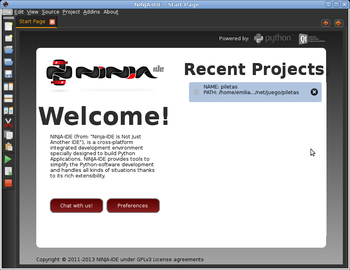
\includegraphics{files/img/u1/ninja-ide.png}
\end{figure}

Un IDE es un entorno que nos facilita las tareas a la hora de programar.
Consiste en la integración de un editor de texto, con características de
resaltado de sintaxis autocompletado -entre otras-, y el intérprete de
Python. Existen cientos de entornos muy buenos, como por ejemplo
\href{https://github.com/spyder-ide/spyder}{Spyder}\footnote{https://github.com/spyder-ide/spyder},
\href{https://www.jetbrains.com/pycharm}{PyCharm}\footnote{https://www.jetbrains.com/pycharm} o
\href{http://ninja-ide.org}{Ninja-IDE}\footnote{http://ninja-ide.org}. Para el presente curso, nos
basaremos en Ninja-IDE, software libre que ha sido desarrollado por la
comunidad de Python Argentina, \href{http://python.org.ar}{PyAr}\footnote{http://python.org.ar}.

Una lista bastante completa sobre las IDEs disponibles pueden
encontrarse en la \href{https://wiki.python.org/moin/IntegratedDevelopmentEnvironments}{wiki oficial de
Python}\footnote{https://wiki.python.org/moin/IntegratedDevelopmentEnvironments}


\section{El primer programa ``Adiós mundo!''}
\label{Unidad01:el-primer-programa-adios-mundo}
El acercamiento inicial a un lenguaje de programación suele ser con el
archiconocido programa ``Hola mundo''. Consiste simmplemente en un
programa que muestra en pantalla ese mensaje.

Renunciando a cualquier pretensión de originalidad comenzaremos del
mismo modo, pero despidiéndonos. Para esto utilizaremos la instrucción
\emph{print()} pasando el mensaje de despedida entre comillas, a continuación
la instrucción.

\begin{Verbatim}[commandchars=\\\{\}]
\PYG{k}{print}\PYG{p}{(}\PYG{l+s}{\PYGZdq{}}\PYG{l+s}{Adios mundo cruel!}\PYG{l+s}{\PYGZdq{}}\PYG{p}{)}
\end{Verbatim}

Podemos probar la intrucción directamente desde el intérprete, creando
con un editor de texto plano un archivo guardado como \code{chau.py} y
luego ejecutándolo desde la terminal haciendo \code{python3 chau.py}, o
bien utilizando un IDE y haciendo todo desde ahí mismo.

Ahora bien, es muchísimo más lo que podemos hacer programando además de
saludar cordialmente. Veamos los elementos de un programa que nos
permitirán realizar tareas más complejas y entretenidas.


\section{Algoritmos computacionales}
\label{Unidad01:algoritmos-computacionales}
En forma simplificada, un programa o software es un conjunto de
instrucciones que la computadora puede ejecutar. Este procedimiento
formado por un conjunto de instrucciones es lo que denominamos algoritmo
computacional. Una analogía a un algoritmo computacional es una receta
de cocina, por ejemplo:

\begin{Verbatim}[commandchars=\\\{\}]
Prender el fuego
Salar la carne
Controlar cada 5 minutos hasta que haya brasas
Poner la carne a la parrilla
Cocinar hasta que esté la carne, controlar cada 5 minutos
Dar vuelta la carne
Cocinar hasta que esté la carne, controlar cada 5 minutos
Si falta sal al probar, salar
\end{Verbatim}

En esta receta se ven una serie de instrucciones que deben ser seguidas
en un determinado orden, en algunos casos contamos con ingredientes,
intrucciones, decisiones y acciones que se repiten. No muy distinto a un
programa de computación, comencemos con algunos \emph{ingredientes} simples
de Python y veamos lo que podemos hacer con ellos.


\section{Elementos de un programa}
\label{Unidad01:elementos-de-un-programa}
A continuación veremos los ingredientes fundamentales de un lenguaje de
programación como Python, para llevar a cabo los ejemplos utilizaremos
el intérprete interactivo mejorado ipython.


\subsection{Números y expresiones}
\label{Unidad01:numeros-y-expresiones}
Frecuentemente requerimos resolver cálculos matemáticos, las operaciones
aritméticas básicas son:
\begin{itemize}
\item {} 
adición: +

\item {} 
sustracción: -

\item {} 
multiplicación: *

\item {} 
división: /

\item {} 
módulo: \%

\item {} 
potencia: **

\item {} 
división entera: //

\end{itemize}

Las operaciones se pueden agrupar con parentesis y tienen precedencia
estándar. Veamos unos ejemplos.

\begin{Verbatim}[commandchars=\\\{\}]
\PYG{l+m+mi}{1}\PYG{o}{/}\PYG{l+m+mi}{3}
\end{Verbatim}

\begin{Verbatim}[commandchars=\\\{\}]
\PYG{l+m+mf}{0.3333333333333333}
\end{Verbatim}

\begin{Verbatim}[commandchars=\\\{\}]
\PYG{l+m+mi}{1}\PYG{o}{/}\PYG{o}{/}\PYG{l+m+mi}{3}
\end{Verbatim}

\begin{Verbatim}[commandchars=\\\{\}]
\PYG{l+m+mi}{0}
\end{Verbatim}

\begin{Verbatim}[commandchars=\\\{\}]
\PYG{l+m+mi}{10}\PYG{o}{\PYGZpc{}}\PYG{l+m+mi}{3}
\end{Verbatim}

\begin{Verbatim}[commandchars=\\\{\}]
\PYG{l+m+mi}{1}
\end{Verbatim}

\begin{Verbatim}[commandchars=\\\{\}]
\PYG{l+m+mi}{4}\PYG{o}{\PYGZpc{}}\PYG{l+m+mi}{2}
\end{Verbatim}

\begin{Verbatim}[commandchars=\\\{\}]
\PYG{l+m+mi}{0}
\end{Verbatim}

El caso de la potencia, también nos sirve para calcularraices. Veamos
una potencia al cubo y luego una raíz cuadrada, equivalente a una
potencia a la 1/2.

\begin{Verbatim}[commandchars=\\\{\}]
\PYG{l+m+mi}{5}\PYG{o}{*}\PYG{o}{*}\PYG{l+m+mi}{3}
\end{Verbatim}

\begin{Verbatim}[commandchars=\\\{\}]
\PYG{l+m+mi}{8}
\end{Verbatim}

\begin{Verbatim}[commandchars=\\\{\}]
\PYG{l+m+mi}{2}\PYG{o}{*}\PYG{o}{*}\PYG{p}{(}\PYG{l+m+mi}{1}\PYG{o}{/}\PYG{l+m+mi}{2}\PYG{p}{)}
\end{Verbatim}

\begin{Verbatim}[commandchars=\\\{\}]
\PYG{l+m+mf}{1.4142135623730951}
\end{Verbatim}

Los datos numéricos que obtenidos en las operaciones previas se
clasifican en reales y enteros, en python se los clasifica como float e
int respectivamente, además existe el tipo complex, para números
complejos.

Utilizando la función type() podemos identificar el tipo de dato.
Veamos:

\begin{Verbatim}[commandchars=\\\{\}]
\PYG{n+nb}{type}\PYG{p}{(}\PYG{l+m+mf}{0.333}\PYG{p}{)}
\end{Verbatim}

\begin{Verbatim}[commandchars=\\\{\}]
\PYG{n+nb}{float}
\end{Verbatim}

\begin{Verbatim}[commandchars=\\\{\}]
\PYG{n+nb}{type}\PYG{p}{(}\PYG{l+m+mi}{3}\PYG{p}{)}
\end{Verbatim}

\begin{Verbatim}[commandchars=\\\{\}]
\PYG{n+nb}{int}
\end{Verbatim}


\subsection{Variables}
\label{Unidad01:variables}
Las variables son contenedores para almacenar información. Por ejemplo,
para elevar un número al cubo podemos utilizar 3 variables, para la base
(\emph{num1}), para el exponenete (\emph{num2}) y para almacenar el \emph{resultado}:

\begin{Verbatim}[commandchars=\\\{\}]
\PYG{n}{num1} \PYG{o}{=} \PYG{l+m+mi}{5}                              \PYG{c}{\PYGZsh{} A num1 se le asigna el valor numérico 5.}
\PYG{n}{num2} \PYG{o}{=} \PYG{l+m+mi}{3}                              \PYG{c}{\PYGZsh{} A num2 se le asigna 3.}
\PYG{n}{resultado} \PYG{o}{=} \PYG{n}{num1}\PYG{o}{*}\PYG{o}{*}\PYG{n}{num2}                \PYG{c}{\PYGZsh{} A resultado se le asigna num1 elevado a num2.}
\PYG{k}{print}\PYG{p}{(}\PYG{l+s}{\PYGZdq{}}\PYG{l+s}{El resultado es}\PYG{l+s}{\PYGZdq{}}\PYG{p}{,} \PYG{n}{resultado}\PYG{p}{)}
\end{Verbatim}

Del código podemos rescatar que el operador igual (=) sirve para asignar
lo que está a la derecha a la variable que se encuentra a la izquierda.


\subsection{Entrada y salida de datos}
\label{Unidad01:entrada-y-salida-de-datos}
Comunicarnos con el entorno


\subsection{Operadores relacionales y lógicos}
\label{Unidad01:operadores-relacionales-y-logicos}

\subsection{Funciones}
\label{Unidad01:funciones}

\subsection{Módulos}
\label{Unidad01:modulos}

\section{Ejercicios}
\label{Unidad01:ejercicios}

\chapter{Estructuras de control}
\label{Unidad02::doc}\label{Unidad02:estructuras-de-control}

\section{Condicionales}
\label{Unidad02:condicionales}

\subsection{if}
\label{Unidad02:if}

\subsection{else}
\label{Unidad02:else}

\subsection{Estructuras anidadas}
\label{Unidad02:estructuras-anidadas}

\subsection{elif}
\label{Unidad02:elif}

\section{Repeticiones}
\label{Unidad02:repeticiones}

\subsection{while}
\label{Unidad02:while}

\section{Ejercicios}
\label{Unidad02:ejercicios}
\begin{Verbatim}[commandchars=\\\{\}]
\PYG{k}{for} \PYG{n}{i} \PYG{o+ow}{in} \PYG{n+nb}{range}\PYG{p}{(}\PYG{l+m+mi}{1}\PYG{p}{,}\PYG{l+m+mi}{10}\PYG{p}{)}\PYG{p}{:}
    \PYG{k}{if} \PYG{n}{i}\PYG{o}{\PYGZpc{}}\PYG{l+m+mi}{2}\PYG{o}{==}\PYG{l+m+mi}{0}\PYG{p}{:}
        \PYG{k}{print}\PYG{p}{(}\PYG{n}{i}\PYG{p}{,}\PYG{l+s}{\PYGZdq{}}\PYG{l+s}{es par}\PYG{l+s}{\PYGZdq{}}\PYG{p}{)}
    \PYG{k}{else}\PYG{p}{:}
        \PYG{k}{print}\PYG{p}{(}\PYG{n}{i}\PYG{p}{,} \PYG{l+s}{\PYGZdq{}}\PYG{l+s}{es impar}\PYG{l+s}{\PYGZdq{}}\PYG{p}{)}
\end{Verbatim}

\begin{Verbatim}[commandchars=\\\{\}]
1 es impar
2 es par
3 es impar
4 es par
5 es impar
6 es par
7 es impar
8 es par
9 es impar
\end{Verbatim}


\chapter{Más estructuras de datos y control}
\label{Unidad03:mas-estructuras-de-datos-y-control}\label{Unidad03::doc}

\section{Listas}
\label{Unidad03:listas}

\section{for}
\label{Unidad03:for}

\section{Manipulando textos con strings}
\label{Unidad03:manipulando-textos-con-strings}

\chapter{Funciones, archivos, diccionarios}
\label{Unidad04::doc}\label{Unidad04:funciones-archivos-diccionarios}

\section{Definiendo funciones}
\label{Unidad04:definiendo-funciones}

\subsection{Variables globales y locales}
\label{Unidad04:variables-globales-y-locales}

\subsubsection{Agrupando el código en módulos}
\label{Unidad04:agrupando-el-codigo-en-modulos}

\section{Números aleatorios}
\label{Unidad04:numeros-aleatorios}

\section{Lectura y escritura de archivos}
\label{Unidad04:lectura-y-escritura-de-archivos}

\section{Diccionarios}
\label{Unidad04:diccionarios}

\chapter{Clases y objetos}
\label{Unidad05::doc}\label{Unidad05:clases-y-objetos}

\chapter{This is a Title}
\label{example::doc}\label{example:this-is-a-title}
That has a paragraph about a main subject and is set when the `='
is at least the same length of the title itself.


\section{Subject Subtitle}
\label{example:subject-subtitle}
Subtitles are set with `-` and are required to have the same length
of the subtitle itself, just like titles.

Lists can be unnumbered like:
\begin{itemize}
\item {} 
Item Foo

\item {} 
Item Bar

\end{itemize}

Or automatically numbered:
\begin{enumerate}
\item {} 
Item 1

\item {} 
Item 2

\end{enumerate}


\section{Inline Markup}
\label{example:inline-markup}
Words can have \emph{emphasis in italics} or be \textbf{bold} and you can define
code samples with back quotes, like when you talk about a command: \code{sudo}
gives you super user powers!


\chapter{Indices and tables}
\label{index:indices-and-tables}\begin{itemize}
\item {} 
\emph{genindex}

\item {} 
\emph{modindex}

\item {} 
\emph{search}

\end{itemize}



\renewcommand{\indexname}{Índice}
\printindex
\end{document}
